\documentclass[11pt,a4paper]{article}

% ============================================================================
% ENCODAGE, LANGUE ET TYPOGRAPHIE (Compatible XeLaTeX & LuaLaTeX)
% ============================================================================
\usepackage{fontspec}
\usepackage[french]{babel}
\frenchsetup{ThinSpaceInFrenchNumbers=true}

% Polices professionnelles disponibles sous Linux / TeX Live
\IfFontExistsTF{TeX Gyre Termes}{
  \setmainfont{TeX Gyre Termes}
}{
  \setmainfont{Latin Modern Roman}
}
\IfFontExistsTF{TeX Gyre Heros}{
  \setsansfont{TeX Gyre Heros}[Scale=MatchLowercase]
}{
  \setsansfont{Latin Modern Sans}[Scale=MatchLowercase]
}
\IfFontExistsTF{TeX Gyre Cursor}{
  \setmonofont{TeX Gyre Cursor}[Scale=MatchLowercase]
}{
  \setmonofont{Latin Modern Mono}[Scale=MatchLowercase]
}

% ============================================================================
% MISE EN PAGE ET GÉOMÉTRIE (Format A4, marges équilibrées)
% ============================================================================
\usepackage[
  a4paper,
  top=2.5cm,
  bottom=2.5cm,
  left=2.5cm,
  right=2.5cm,
  headheight=22pt
]{geometry}

\usepackage{setspace}
\setstretch{1.12}
\setlength{\parskip}{0.45em}
\setlength{\parindent}{0pt}

% ============================================================================
% COULEURS ET ÉLÉMENTS GRAPHIQUES
% ============================================================================
\usepackage[table]{xcolor}
\definecolor{BleuInstitutionnel}{HTML}{1F3A5F}
\definecolor{BleuSecondaire}{HTML}{2E5B88}
\definecolor{GrisFonce}{HTML}{2C3E50}
\definecolor{GrisClair}{HTML}{F4F6F9}
\definecolor{GrisBordure}{HTML}{D0D7DE}

\usepackage{graphicx}
\usepackage{float}
\usepackage{pdflscape}
\usepackage{caption}
\captionsetup{
  font=small,
  labelfont={bf,color=BleuInstitutionnel},
  textfont={it},
  skip=8pt
}

% ============================================================================
% TABLEAUX
% ============================================================================
\usepackage{booktabs}
\usepackage{tabularx}
\usepackage{longtable}
\usepackage{array}
\usepackage{multirow}

\newcolumntype{L}[1]{>{\raggedright\arraybackslash}p{#1}}
\newcolumntype{Y}{>{\raggedright\arraybackslash}X}

\renewcommand{\arraystretch}{1.35}

% ============================================================================
% LISTES ET TITRES DE SECTIONS
% ============================================================================
\usepackage{enumitem}
\setlist[itemize]{topsep=3pt, itemsep=2pt, leftmargin=1.5em, label=\textcolor{BleuInstitutionnel}{\textbullet}}
\setlist[enumerate]{topsep=3pt, itemsep=3pt, leftmargin=1.8em}

\usepackage{titlesec}
\titleformat{\section}
  {\normalfont\Large\bfseries\sffamily\color{BleuInstitutionnel}}
  {\thesection.}{0.6em}{}
  [\vspace{2pt}\titlerule]

\titleformat{\subsection}
  {\normalfont\large\bfseries\sffamily\color{BleuSecondaire}}
  {\thesubsection.}{0.5em}{}

\titleformat{\subsubsection}
  {\normalfont\normalsize\bfseries\sffamily\color{GrisFonce}}
  {\thesubsubsection.}{0.5em}{}

\titlespacing*{\section}{0pt}{1.8ex plus 0.5ex minus .2ex}{1.2ex plus .2ex}
\titlespacing*{\subsection}{0pt}{1.4ex plus 0.4ex minus .2ex}{0.8ex plus .2ex}
\titlespacing*{\subsubsection}{0pt}{1.1ex plus 0.3ex minus .1ex}{0.5ex plus .1ex}

% ============================================================================
% EN-TÊTES ET PIEDS DE PAGE DISCRETS
% ============================================================================
\usepackage{fancyhdr}
\usepackage{lastpage}
\pagestyle{fancy}
\fancyhf{}
\fancyhead[L]{\footnotesize\sffamily\textcolor{GrisFonce}{Analyse fonctionnelle préliminaire — Suivi des dépenses budgétaires}}
\fancyhead[R]{\footnotesize\sffamily\textcolor{GrisFonce}{Document de travail — V1.0}}
\fancyfoot[L]{\footnotesize\sffamily\textcolor{GrisFonce}{Système d'information de gestion administrative et financière}}
\fancyfoot[R]{\footnotesize\sffamily\textcolor{GrisFonce}{Page \thepage\ sur \pageref*{LastPage}}}
\renewcommand{\headrulewidth}{0.4pt}
\renewcommand{\footrulewidth}{0.4pt}
\renewcommand{\headrule}{\hbox to\headwidth{\color{GrisBordure}\leaders\hrule height \headrulewidth\hfill}}
\renewcommand{\footrule}{\hbox to\headwidth{\color{GrisBordure}\leaders\hrule height \footrulewidth\hfill}}

% ============================================================================
% ENCADRÉS MÉTHODOLOGIQUES SOBRES
% ============================================================================
\usepackage{tcolorbox}
\newtcolorbox{encadre}[1]{
  colback=GrisClair,
  colframe=BleuInstitutionnel,
  boxrule=0.6pt,
  leftrule=3pt,
  arc=1.5pt,
  fonttitle=\bfseries\sffamily\small,
  coltitle=white,
  colbacktitle=BleuInstitutionnel,
  title=#1,
  top=6pt,
  bottom=6pt,
  left=8pt,
  right=8pt
}

% ============================================================================
% HYPERLIENS
% ============================================================================
\usepackage[
  colorlinks=true,
  linkcolor=BleuInstitutionnel,
  urlcolor=BleuSecondaire,
  citecolor=BleuInstitutionnel,
  pdftitle={Analyse fonctionnelle preliminaire - Application de suivi des depenses budgetaires},
  pdfauthor={Architecture des Systemes d'Information}
]{hyperref}

% ============================================================================
% CORPS DU DOCUMENT
% ============================================================================
\begin{document}

% 1. Page de garde
\begin{titlepage}
\thispagestyle{empty}

\begin{center}
  % Bandeau supérieur institutionnel
  {\color{BleuInstitutionnel}\rule{\linewidth}{2pt}}
  \vspace{0.3cm}

  {\large\sffamily\bfseries\textcolor{BleuInstitutionnel}{SYSTÈME D'INFORMATION DE GESTION ADMINISTRATIVE ET FINANCIÈRE}}\\[0.2cm]
  {\normalsize\sffamily\textcolor{GrisFonce}{Dématérialisation de la chaîne de la dépense budgétaire}}

  \vspace{0.3cm}
  {\color{BleuInstitutionnel}\rule{\linewidth}{0.8pt}}

  \vspace{3.2cm}

  % Titre principal
  {\fontsize{22}{28}\selectfont\sffamily\bfseries\textcolor{BleuInstitutionnel}{Analyse fonctionnelle préliminaire}}\\[0.5cm]
  {\fontsize{16}{22}\selectfont\sffamily\textcolor{BleuSecondaire}{Application de suivi des dépenses budgétaires}}

  \vspace{1.2cm}
  {\color{GrisBordure}\rule{0.45\linewidth}{1pt}}
  \vspace{1.2cm}

  {\normalsize\itshape\textcolor{GrisFonce}{%
    Structuration du processus métier, identification des responsabilités des acteurs\\
    et modélisation générale des cas d'utilisation (UML)%
  }}

  \vfill

  % Cartouche d'identification du document
  \begin{tabularx}{0.92\linewidth}{L{4.5cm} Y}
    \toprule
    \textbf{\sffamily\textcolor{BleuInstitutionnel}{Nature du document}} & Document de travail — Cadrage fonctionnel initial \\
    \textbf{\sffamily\textcolor{BleuInstitutionnel}{Version}} & 1.0 (Version soumise à validation métier) \\
    \textbf{\sffamily\textcolor{BleuInstitutionnel}{Auteur}} & Architecte logiciel senior — Conception SI \& Modélisation UML \\
    \textbf{\sffamily\textcolor{BleuInstitutionnel}{Destinataire}} & Responsable du projet (Maîtrise d'ouvrage métier) \\
    \textbf{\sffamily\textcolor{BleuInstitutionnel}{Source documentaire}} & Notes issues de la réunion de cadrage initial \\
    \textbf{\sffamily\textcolor{BleuInstitutionnel}{Périmètre}} & De l'expression du besoin à la transmission au comptable public \\
    \bottomrule
  \end{tabularx}

  \vspace{1.2cm}
  {\footnotesize\sffamily\textcolor{GrisFonce}{\today}}
\end{center}

\end{titlepage}
\newpage


% Table des matières
\thispagestyle{fancy}
\tableofcontents
\newpage

% 2. Introduction
\section{Introduction}

\subsection{Objet du document}

Le présent document constitue la première analyse fonctionnelle de l'application de suivi des dépenses budgétaires. Il formalise et structure les éléments recueillis lors de la réunion initiale organisée avec le responsable du projet.

Son objectif est de fournir à la maîtrise d'ouvrage une représentation claire, partagée et vérifiable du fonctionnement attendu du futur système, avant d'engager les travaux de modélisation des données et de conception technique.

\subsection{Démarche méthodologique et périmètre d'analyse}

Conformément aux principes d'ingénierie des systèmes d'information administratifs et financiers, cette première étape se concentre exclusivement sur la vision fonctionnelle externe du système :

\begin{itemize}
  \item la structuration du processus métier de bout en bout, depuis l'expression du besoin jusqu'à la transmission du dossier d'ordonnancement au comptable public ;
  \item l'identification précise des acteurs intervenant dans la chaîne de la dépense et la délimitation de leurs responsabilités respectives ;
  \item la définition des fonctionnalités attendues du système à travers un diagramme général des cas d'utilisation conforme à la norme UML ;
  \item le recensement des zones d'incertitude et des règles de gestion qui devront être arbitrées par le responsable du projet.
\end{itemize}

\begin{encadre}{Principe de rigueur documentaire}
Afin de garantir la fidélité de l'analyse aux besoins exprimés, ce rapport distingue strictement :
\begin{enumerate}
  \item \textbf{les faits établis}, directement issus des notes de la réunion de cadrage ;
  \item \textbf{les hypothèses de structuration}, introduites uniquement pour organiser logiquement l'enchaînement des opérations ;
  \item \textbf{les points à valider}, qui font l'objet d'un questionnaire dédié en section 8 et ne doivent pas être considérés comme des règles métier définitives.
\end{enumerate}
Aucune responsabilité ni étape supplémentaire n'a été extrapolée au-delà des éléments communiqués.
\end{encadre}


% 3. Contexte et objectifs du projet
\section{Contexte et objectifs du projet}

\subsection{Contexte opérationnel}

L'exécution d'une dépense budgétaire repose sur une chaîne procédurale réglementée qui mobilise plusieurs intervenants internes et externes : l'ordonnateur, les fournisseurs, le contrôleur financier, le comptable matière et le comptable public. Cette organisation s'appuie sur le principe de séparation des fonctions d'initiative et d'engagement, de contrôle budgétaire préalable, de réception physique des biens et de prise en charge comptable.

En l'absence d'un outil fédérateur, la multiplicité des intervenants et des pièces justificatives expose le traitement des dossiers à des risques de lenteur dans la transmission de l'information, de perte de visibilité sur l'état d'avancement des demandes et de ressaisies multiples.

\subsection{Objectifs de l'application}

Le projet vise à concevoir une application informatique dédiée au suivi du processus de dépense budgétaire, depuis l'expression initiale du besoin jusqu'à la transmission du dossier d'ordonnancement au comptable public.

Trois objectifs opérationnels structurent cette démarche :

\begin{enumerate}
  \item \textbf{Structurer les interventions des différents acteurs :} attribuer à chaque intervenant un périmètre d'action clairement délimité dans le système, conforme à ses attributions administratives et financières.
  \item \textbf{Faciliter la circulation des dossiers :} fluidifier la transmission des projets d'actes, des informations de livraison, des factures, des pièces justificatives et des dossiers d'ordonnancement entre les acteurs successifs.
  \item \textbf{Assurer le suivi et la traçabilité des opérations :} permettre le suivi de l'évolution des demandes et conserver la trace des contrôles, visas, réceptions et signatures intervenus tout au long du cycle de vie de la dépense.
\end{enumerate}

\subsection{Limites de la présente phase d'étude}

Ce document s'inscrit dans une phase d'étude préliminaire. À ce stade :
\begin{itemize}
  \item il ne définit pas encore les objets métier détaillés, leurs attributs ou le modèle de données ;
  \item il ne préjuge d'aucun choix d'architecture logicielle ou d'infrastructure technique ;
  \item il s'arrête, conformément aux éléments recueillis, à la réception du dossier d'ordonnancement par le comptable public, sans couvrir les opérations ultérieures de règlement effectif ou de tenue de la comptabilité générale.
\end{itemize}


% 4. Présentation du processus métier
\section{Présentation du processus métier}

\subsection{Vue d'ensemble et structuration du cycle de la dépense}

L'analyse des opérations décrites lors de la réunion de cadrage permet de structurer le traitement d'une dépense budgétaire en quatre grandes phases successives :

\begin{enumerate}
  \item \textbf{Phase 1 — Expression du besoin et soumission :} formalisation du besoin par l'ordonnateur, consultation des besoins ouverts par les fournisseurs et dépôt des soumissions.
  \item \textbf{Phase 2 — Engagement juridique et contrôle budgétaire préalable :} préparation du projet d'acte juridique par l'ordonnateur, examen et contrôles par le contrôleur financier (réservation des crédits, quitus sur le classement en nature économique, visa), puis signature de l'acte juridique par l'ordonnateur.
  \item \textbf{Phase 3 — Exécution des livraisons et réception matière :} réalisation des livraisons par le fournisseur, prise en charge et constatation des produits livrés par le comptable matière, délivrance du procès-verbal de réception au fournisseur et information de l'ordonnateur.
  \item \textbf{Phase 4 — Facturation, liquidation et ordonnancement :} introduction de la demande de paiement accompagnée des factures et pièces justificatives par le fournisseur, enregistrement et validation des factures par l'ordonnateur, liquidation de la dépense, génération et signature du projet d'ordonnancement par l'ordonnateur, puis contrôle, signature et transmission du dossier d'ordonnancement par le contrôleur financier au comptable public.
\end{enumerate}

\subsection{Description détaillée des étapes de traitement}

\subsubsection{Étape 1 : Expression du besoin et mise en concurrence}
Le processus débute lorsque l'\textbf{ordonnateur} exprime un besoin au sein du système sous la forme de lignes de besoin précisant la matière, les quantités demandées et les spécifications techniques (sans fixation de prix unitaire au niveau des lignes, cette valorisation incombant exclusivement aux prestataires). Les expressions de besoin ouvertes à la soumission sont rendues accessibles aux \textbf{fournisseurs}. Ces derniers consultent les besoins publiés et déposent une soumission totale en renseignant leur prix unitaire proposé pour chaque ligne de besoin, consolidant ainsi le montant financier global de leur offre.

\subsubsection{Étape 2 : Préparation, contrôle préalable et signature de l'acte juridique}
L'\textbf{ordonnateur} prépare le projet d'acte juridique matérialisant l'engagement de la dépense et le soumet au \textbf{contrôleur financier}.

À la réception de ce projet, le \textbf{contrôleur financier} intervient à trois niveaux :
\begin{itemize}
  \item il effectue la réservation des crédits correspondants ;
  \item il donne le quitus sur le classement des matières dans les natures économiques ;
  \item il examine et vise le projet d'acte juridique.
\end{itemize}
Une fois les contrôles requis effectués et le visa obtenu, l'\textbf{ordonnateur} signe l'acte juridique.

\subsubsection{Étape 3 : Livraison et réception par le comptable matière}
En exécution de l'engagement, le \textbf{fournisseur} effectue les livraisons. Le \textbf{comptable matière} prend en charge ces livraisons et constate les produits effectivement livrés. À l'issue de cette constatation, le comptable matière réalise deux opérations de communication :
\begin{itemize}
  \item il établit et délivre au \textbf{fournisseur} un procès-verbal de réception ;
  \item il informe l'\textbf{ordonnateur} des livraisons effectuées (l'ordonnateur reçoit ainsi les informations relatives aux livraisons).
\end{itemize}

\subsubsection{Étape 4 : Demande de paiement, liquidation et projet d'ordonnancement}
Le \textbf{fournisseur} introduit une demande de paiement dans le système en soumettant les factures ainsi que les pièces justificatives requises. Il dispose par ailleurs de la capacité de suivre l'évolution de ses demandes tout au long du traitement.

Sur la base des informations de livraison reçues du comptable matière et des éléments soumis par le fournisseur, l'\textbf{ordonnateur} :
\begin{itemize}
  \item enregistre et valide les factures ;
  \item procède à la liquidation de la dépense ;
  \item génère un projet d'ordonnancement de paiement ;
  \item signe ce projet d'ordonnancement et le transmet au \textbf{contrôleur financier}.
\end{itemize}

\subsubsection{Étape 5 : Contrôle de l'ordonnancement et transmission au comptable public}
Le \textbf{contrôleur financier} reçoit le projet d'ordonnancement transmis par l'ordonnateur. Il effectue les contrôles nécessaires sur le dossier, puis signe et transmet le dossier d'ordonnancement au \textbf{comptable public}.

Le \textbf{comptable public} reçoit le dossier d'ordonnancement transmis par le contrôleur financier, ce qui clôt le périmètre fonctionnel décrit à ce stade.

\subsection{Synthèse des interactions entre acteurs}

Le tableau \ref{tab:interactions} récapitule les flux d'échanges fonctionnels identifiés entre les acteurs tout au long du circuit de la dépense.

\begin{table}[H]
\centering
\small
\caption{Principales interactions entre les acteurs du processus}
\label{tab:interactions}
\begin{tabularx}{\linewidth}{L{1.1cm} L{3.2cm} L{3.2cm} Y}
\toprule
\textbf{\sffamily Réf.} & \textbf{\sffamily Acteur émetteur} & \textbf{\sffamily Acteur récepteur} & \textbf{\sffamily Objet de l'interaction} \\
\midrule
I01 & Ordonnateur & Fournisseur & Mise à disposition des expressions de besoin ouvertes à la soumission. \\
I02 & Fournisseur & Ordonnateur & Dépôt d'une soumission en réponse à une expression de besoin. \\
I03 & Ordonnateur & Contrôleur financier & Transmission du projet d'acte juridique pour examen et visa. \\
I04 & Contrôleur financier & Ordonnateur & Retour du projet d'acte juridique visé (après réservation des crédits et quitus sur le classement économique) pour signature. \\
I05 & Fournisseur & Comptable matière & Réalisation physique de la livraison des produits commandés. \\
I06 & Comptable matière & Fournisseur & Délivrance du procès-verbal de réception constatant les produits livrés. \\
I07 & Comptable matière & Ordonnateur & Transmission des informations relatives aux livraisons constatées. \\
I08 & Fournisseur & Ordonnateur & Introduction de la demande de paiement accompagnée des factures et pièces justificatives. \\
I09 & Ordonnateur & Contrôleur financier & Transmission du projet d'ordonnancement de paiement signé. \\
I10 & Contrôleur financier & Comptable public & Transmission du dossier d'ordonnancement contrôlé et signé. \\
\bottomrule
\end{tabularx}
\end{table}

\subsection{Documents et dossiers explicitement mentionnés}

L'analyse stricte des notes de cadrage met en évidence sept supports documentaires ou dossiers échangés au cours du processus :

\begin{table}[H]
\centering
\small
\caption{Documents et dossiers mentionnés dans l'expression de besoin initiale}
\label{tab:documents}
\begin{tabularx}{\linewidth}{L{4.2cm} L{3.3cm} L{3.3cm} Y}
\toprule
\textbf{\sffamily Document / Dossier} & \textbf{\sffamily Producteur / Émetteur} & \textbf{\sffamily Destinataire(s)} & \textbf{\sffamily Étape associée} \\
\midrule
Expression de besoin & Ordonnateur & Fournisseurs & Expression du besoin \\
Projet d'acte juridique / Acte juridique signé & Ordonnateur (visé par le Contrôleur financier) & Contrôleur financier, Fournisseur & Engagement juridique \\
Procès-verbal de réception & Comptable matière & Fournisseur (et information de l'Ordonnateur) & Réception des livraisons \\
Demande de paiement & Fournisseur & Ordonnateur & Facturation \\
Factures & Fournisseur & Ordonnateur & Facturation et liquidation \\
Pièces justificatives & Fournisseur & Ordonnateur & Facturation et liquidation \\
Projet / Dossier d'ordonnancement & Ordonnateur, puis Contrôleur financier & Contrôleur financier, puis Comptable public & Ordonnancement \\
\bottomrule
\end{tabularx}
\end{table}

\subsection{Première identification des zones d'ombre et ambiguïtés du processus}

La reconstitution du circuit global fait apparaître plusieurs discontinuités ou imprécisions dans les notes initiales, qui devront être levées avec le responsable du projet :

\begin{itemize}
  \item \textbf{Transition entre les soumissions et le projet d'acte juridique :} le fournisseur soumissionne à une expression de besoin et l'ordonnateur prépare ensuite un projet d'acte juridique, mais l'étape intermédiaire d'évaluation des offres et de sélection du fournisseur retenu n'est pas décrite.
  \item \textbf{Ordonnancement chronologique des actes du contrôleur financier lors de l'engagement :} les notes mentionnent la réservation des crédits, le quitus sur le classement des matières dans les natures économiques et l'examen/visa du projet d'acte juridique, sans préciser si ces trois opérations sont réalisées simultanément lors de la soumission du projet d'acte juridique ou lors de jalons distincts.
  \item \textbf{Notification de l'acte juridique signé au fournisseur :} les notes indiquent que l'ordonnateur signe l'acte juridique après les contrôles requis et que le fournisseur effectue les livraisons, sans expliciter la manière dont l'acte signé (bon de commande, marché ou contrat) est notifié au fournisseur pour déclencher la livraison.
  \item \textbf{Articulation entre le procès-verbal de réception et la demande de paiement :} le comptable matière délivre un procès-verbal de réception au fournisseur et informe l'ordonnateur des livraisons ; de son côté, le fournisseur soumet une demande de paiement avec factures et pièces justificatives. Il convient de confirmer si le procès-verbal de réception fait partie des pièces justificatives jointes par le fournisseur ou s'il est directement rattaché au dossier par le système.
  \item \textbf{Absence de circuits de rejet ou de demande de régularisation :} le processus décrit uniquement le scénario nominal (validation à chaque étape). Le comportement attendu en cas de refus de visa, de livraison non conforme ou de facture erronée n'est pas encore spécifié.
  \item \textbf{Fin du processus chez le comptable public :} le comptable public reçoit le dossier d'ordonnancement, mais aucune opération de prise en charge, de contrôle de régularité, de paiement ou de retour d'information vers l'ordonnateur et le fournisseur n'est mentionnée.
\end{itemize}


% 5. Identification des acteurs
\section{Identification des acteurs}

\subsection{Recensement des acteurs du périmètre}

L'analyse des notes de cadrage permet d'identifier cinq acteurs intervenant directement dans le système de suivi des dépenses budgétaires :

\begin{enumerate}
  \item \textbf{L'Ordonnateur} (acteur interne) : autorité administrative à l'initiative de la dépense, responsable de l'engagement juridique, de la liquidation et de l'ordonnancement.
  \item \textbf{Le Fournisseur} (acteur externe) : opérateur économique qui répond aux expressions de besoin, exécute les livraisons et sollicite le règlement de ses prestations.
  \item \textbf{Le Contrôleur financier} (acteur interne ou organe de contrôle budgétaire) : autorité chargée du contrôle a priori de la régularité budgétaire, de la disponibilité des crédits et de la conformité de l'imputation économique, tant au stade de l'engagement qu'au stade de l'ordonnancement.
  \item \textbf{Le Comptable matière} (acteur interne) : agent chargé de la réception physique des biens livrés, de la constatation qualitative et quantitative des produits et de la certification de l'entrée en matière.
  \item \textbf{Le Comptable public} (acteur interne / Trésor) : destinataire final du dossier d'ordonnancement validé et signé par le contrôleur financier dans le périmètre actuel de l'application.
\end{enumerate}

\subsection{Distinction entre responsabilités métier et droits d'accès applicatifs}

Dans la conception d'un système d'information administratif et financier, il est essentiel de ne pas confondre la \textbf{responsabilité métier} d'un acteur avec les \textbf{droits d'accès techniques} (profils d'habilitation) qui seront configurés dans l'application.

\begin{table}[H]
\centering
\small
\caption{Distinction entre responsabilité métier et profil d'accès applicatif}
\label{tab:distinction_metier_acces}
\begin{tabularx}{\linewidth}{L{3.5cm} Y Y}
\toprule
\textbf{\sffamily Dimension} & \textbf{\sffamily Responsabilité métier} & \textbf{\sffamily Droit d'accès à l'application} \\
\midrule
\textbf{Définition} & Attribution juridique, administrative ou comptable conférée à une fonction par la réglementation (ex. engager l'organisme, accorder un quitus, certifier le service fait, signer un ordonnancement). & Permission technique accordée à un compte utilisateur pour consulter un écran, saisir un formulaire, téléverser un document ou déclencher une transition d'état. \\
\textbf{Portée de l'engagement} & Engage la responsabilité personnelle et fonctionnelle du titulaire du rôle (signature d'un acte juridique, visa financier, procès-verbal de réception). & Permet l'exécution matérielle d'une tâche dans le logiciel, éventuellement par délégation ou préparation de dossier. \\
\textbf{Modélisation UML} & Représentée par l'\textbf{Acteur} (rôle fonctionnel externe interagissant avec le système pour atteindre un objectif métier à valeur ajoutée). & Représentée ultérieurement dans la matrice de sécurité et de contrôle d'accès (gestion des comptes, profils de saisie, profils de validation). \\
\textbf{Exemple concret dans le projet} & L'\textbf{Ordonnateur} porte la responsabilité de préparer et signer l'acte juridique ainsi que le projet d'ordonnancement. & En pratique, des agents des services gestionnaires pourront disposer d'un droit de \emph{préparation/saisie}, tandis que le droit de \emph{signature/validation} sera restreint à l'ordonnateur habilité. \\
\bottomrule
\end{tabularx}
\end{table}

Dans la suite de ce document et dans le diagramme des cas d'utilisation UML, chaque acteur représente un \textbf{rôle métier cohérent} au sens de la réglementation budgétaire, indépendamment du découpage organisationnel interne des services qui sera précisé lors des ateliers détaillés.


% 6. Description des responsabilités
\section{Description des responsabilités}

\subsection{Détail des attributions par acteur}

Conformément aux éléments communiqués lors de la réunion de cadrage, les responsabilités métier et les opérations associées à chaque acteur s'établissent comme suit :

\subsubsection{1. L'Ordonnateur}
L'ordonnateur assure le pilotage administratif de la dépense de son initialisation jusqu'à l'ordre de payer. Ses attributions portent sur :
\begin{itemize}
  \item l'initiative de la dépense par l'expression du besoin ;
  \item la formalisation de l'engagement juridique (préparation du projet d'acte juridique, soumission au contrôleur financier, puis signature de l'acte après obtention des contrôles requis) ;
  \item la prise en compte de l'exécution physique à travers la réception des informations relatives aux livraisons transmises par le comptable matière ;
  \item la vérification des droits du créancier et l'arrêté du montant de la dépense (enregistrement et validation des factures, réalisation de la liquidation) ;
  \item l'émission de l'ordre de paiement (génération du projet d'ordonnancement de paiement, signature et transmission au contrôleur financier).
\end{itemize}

\subsubsection{2. Le Fournisseur}
Le fournisseur intervient comme cocontractant de l'administration. Ses interventions couvrent :
\begin{itemize}
  \item la participation à la mise en concurrence (consultation des expressions de besoin ouvertes à la soumission et dépôt d'une soumission) ;
  \item l'exécution matérielle de la commande (réalisation des livraisons et réception du procès-verbal établi par le comptable matière) ;
  \item la demande de règlement financier (introduction d'une demande de paiement accompagnée de la soumission des factures et des pièces justificatives) ;
  \item la consultation de l'avancement du traitement (suivi de l'évolution de ses demandes).
\end{itemize}

\subsubsection{3. Le Contrôleur financier}
Le contrôleur financier garantit la régularité budgétaire et financière des opérations à deux moments clés du processus :
\begin{itemize}
  \item \textbf{lors de l'engagement juridique :} il effectue la réservation des crédits, donne le quitus sur le classement des matières dans les natures économiques, et examine puis vise les projets d'actes juridiques soumis par l'ordonnateur ;
  \item \textbf{lors de l'ordonnancement :} il reçoit les projets d'ordonnancement signés par l'ordonnateur, effectue les contrôles nécessaires, puis signe et transmet les dossiers d'ordonnancement au comptable public.
\end{itemize}

\subsubsection{4. Le Comptable matière}
Le comptable matière assure le contrôle physique et patrimonial des biens livrés :
\begin{itemize}
  \item il prend en charge les livraisons effectuées par le fournisseur ;
  \item il constate les produits effectivement livrés ;
  \item il informe l'ordonnateur des livraisons réalisées ;
  \item il établit et délivre au fournisseur un procès-verbal de réception.
\end{itemize}

\subsubsection{5. Le Comptable public}
Dans les limites des informations communiquées à ce stade :
\begin{itemize}
  \item il reçoit les dossiers d'ordonnancement signés et transmis par le contrôleur financier.
\end{itemize}
\emph{Nota : conformément aux règles méthodologiques retenues, aucune responsabilité supplémentaire (telle que le contrôle de régularité comptable ou le décaissement) n'est ajoutée sans confirmation préalable du responsable du projet.}

\subsection{Tableau synthétique des acteurs et de leurs responsabilités}

Le tableau \ref{tab:acteurs_synthese} présente la synthèse structurée des cinq acteurs, en distinguant leur rôle métier global, leurs responsabilités métier, les opérations qu'ils réalisent dans le système et les acteurs avec lesquels ils interagissent.

\begin{landscape}
\small
\begin{longtable}{L{2.8cm} L{3.6cm} L{5.8cm} L{6.2cm} L{3.8cm}}
\caption{Tableau synthétique des acteurs, rôles, responsabilités métier, opérations et interactions}
\label{tab:acteurs_synthese} \\
\toprule
\textbf{\sffamily Acteur} &
\textbf{\sffamily Rôle dans le processus} &
\textbf{\sffamily Principales responsabilités métier} &
\textbf{\sffamily Principales opérations réalisées} &
\textbf{\sffamily Autres acteurs en interaction} \\
\midrule
\endfirsthead

\multicolumn{5}{l}{\footnotesize\itshape Suite du tableau \ref{tab:acteurs_synthese} — Acteurs et responsabilités} \\
\toprule
\textbf{\sffamily Acteur} &
\textbf{\sffamily Rôle dans le processus} &
\textbf{\sffamily Principales responsabilités métier} &
\textbf{\sffamily Principales opérations réalisées} &
\textbf{\sffamily Autres acteurs en interaction} \\
\midrule
\endhead

\bottomrule
\endfoot

\textbf{Ordonnateur} &
Initiateur de la dépense, autorité d'engagement juridique, de liquidation et d'ordonnancement &
\begin{itemize}[leftmargin=1em, nosep]
  \item Définition officielle du besoin
  \item Engagement juridique de l'organisme après visa préalable
  \item Vérification de la réalité de la dette et arrêté du montant exact de la dépense (liquidation)
  \item Émission et signature de l'ordre de payer (projet d'ordonnancement)
\end{itemize} &
\begin{itemize}[leftmargin=1em, nosep]
  \item Exprimer un besoin
  \item Préparer le projet d'acte juridique
  \item Soumettre le projet au contrôleur financier
  \item Signer l'acte juridique après les contrôles requis
  \item Recevoir les informations relatives aux livraisons
  \item Enregistrer et valider les factures
  \item Procéder à la liquidation
  \item Générer un projet d'ordonnancement de paiement
  \item Signer et transmettre le projet au contrôleur financier
\end{itemize} &
\begin{itemize}[leftmargin=1em, nosep]
  \item Fournisseur
  \item Contrôleur financier
  \item Comptable matière
\end{itemize} \\
\midrule

\textbf{Fournisseur} &
Opérateur économique soumissionnaire, exécutant des livraisons et créancier &
\begin{itemize}[leftmargin=1em, nosep]
  \item Formulation d'une offre commerciale en réponse à un besoin
  \item Exécution conforme des livraisons convenues
  \item Justification de sa créance en vue du paiement
\end{itemize} &
\begin{itemize}[leftmargin=1em, nosep]
  \item Consulter les expressions de besoin ouvertes à la soumission
  \item Soumissionner à une expression de besoin
  \item Effectuer les livraisons
  \item Introduire une demande de paiement
  \item Soumettre les factures et les pièces justificatives
  \item Suivre l'évolution de ses demandes
\end{itemize} &
\begin{itemize}[leftmargin=1em, nosep]
  \item Ordonnateur
  \item Comptable matière
\end{itemize} \\
\midrule

\textbf{Contrôleur financier} &
Autorité de contrôle budgétaire a priori sur l'engagement et l'ordonnancement &
\begin{itemize}[leftmargin=1em, nosep]
  \item Garantie de la disponibilité et du blocage des crédits budgétaires
  \item Validation de l'exactitude de l'imputation en nature économique (quitus)
  \item Contrôle de régularité et visa préalable des projets d'actes juridiques
  \item Contrôle final, signature et transmission des dossiers d'ordonnancement
\end{itemize} &
\begin{itemize}[leftmargin=1em, nosep]
  \item Effectuer la réservation des crédits
  \item Donner le quitus sur le classement des matières dans les natures économiques
  \item Examiner et viser les projets d'actes juridiques
  \item Recevoir les projets d'ordonnancement
  \item Effectuer les contrôles nécessaires
  \item Signer et transmettre les dossiers au comptable public
\end{itemize} &
\begin{itemize}[leftmargin=1em, nosep]
  \item Ordonnateur
  \item Comptable public
\end{itemize} \\
\midrule

\textbf{Comptable matière} &
Garant de la réception physique et de la constatation des biens livrés &
\begin{itemize}[leftmargin=1em, nosep]
  \item Réception matérielle et vérification effective des biens livrés
  \item Attestation officielle de la livraison par procès-verbal
  \item Information de l'ordonnateur pour permettre la liquidation
\end{itemize} &
\begin{itemize}[leftmargin=1em, nosep]
  \item Prendre en charge les livraisons
  \item Constater les produits effectivement livrés
  \item Informer l'ordonnateur des livraisons
  \item Établir et délivrer au fournisseur un procès-verbal de réception
\end{itemize} &
\begin{itemize}[leftmargin=1em, nosep]
  \item Fournisseur
  \item Ordonnateur
\end{itemize} \\
\midrule

\textbf{Comptable public} &
Destinataire institutionnel des dossiers d'ordonnancement validés &
\begin{itemize}[leftmargin=1em, nosep]
  \item Réception officielle des dossiers d'ordonnancement transmis après contrôle financier (dans la limite du périmètre documenté)
\end{itemize} &
\begin{itemize}[leftmargin=1em, nosep]
  \item Recevoir les dossiers d'ordonnancement transmis par le contrôleur financier
\end{itemize} &
\begin{itemize}[leftmargin=1em, nosep]
  \item Contrôleur financier
\end{itemize} \\
\end{longtable}
\end{landscape}


% 7. Présentation des principaux cas d'utilisation
\section{Présentation des principaux cas d'utilisation}

\subsection{Organisation par domaines fonctionnels}

Afin d'offrir une lecture claire et modulaire du système sans surcharger la représentation graphique, les cas d'utilisation ont été regroupés en quatre grands domaines fonctionnels correspondant aux phases majeures du cycle de vie de la dépense :

\begin{enumerate}
  \item \textbf{Domaine 1 — Expression du besoin et mise en concurrence} ;
  \item \textbf{Domaine 2 — Engagement juridique et contrôle budgétaire préalable} ;
  \item \textbf{Domaine 3 — Exécution des livraisons et réception matière} ;
  \item \textbf{Domaine 4 — Facturation, liquidation et ordonnancement}.
\end{enumerate}

Chaque cas d'utilisation traduit un service fonctionnel complet rendu par le système à un ou plusieurs acteurs, à l'exclusion de toute fonction purement technique (telle que l'authentification ou le paramétrage).

\subsection{Catalogue des cas d'utilisation par domaine}

\begin{table}[H]
\centering
\small
\caption{Catalogue structuré des cas d'utilisation du système}
\label{tab:catalogue_uc}
\begin{tabularx}{\linewidth}{L{1.2cm} L{5.0cm} L{3.6cm} Y}
\toprule
\textbf{\sffamily Code} & \textbf{\sffamily Intitulé du cas d'utilisation} & \textbf{\sffamily Acteur(s) participant(s)} & \textbf{\sffamily Description fonctionnelle synthétique} \\
\midrule
\multicolumn{4}{l}{\cellcolor{GrisClair}\textbf{\sffamily\textcolor{BleuInstitutionnel}{Domaine 1 — Expression du besoin et mise en concurrence}}} \\
\midrule
UC01 & Exprimer un besoin & Ordonnateur & Enregistrer et publier dans le système une expression de besoin. \\
UC02 & Consulter les expressions de besoin ouvertes & Fournisseur & Parcourir et consulter le détail des expressions de besoin ouvertes à la soumission. \\
UC03 & Soumissionner à une expression de besoin & Fournisseur & Déposer une offre en réponse à une expression de besoin ouverte. \\
\midrule
\multicolumn{4}{l}{\cellcolor{GrisClair}\textbf{\sffamily\textcolor{BleuInstitutionnel}{Domaine 2 — Engagement juridique et contrôle budgétaire préalable}}} \\
\midrule
UC04 & Préparer et soumettre le projet d'acte juridique & Ordonnateur & Élaborer le projet d'acte juridique et le transmettre pour contrôle au contrôleur financier. \\
UC05 & Signer l'acte juridique & Ordonnateur & Apposer la signature de l'ordonnateur sur l'acte juridique après obtention des contrôles et visas requis. \\
UC06 & Examiner et viser le projet d'acte juridique & Contrôleur financier & Instruire le projet d'acte juridique soumis par l'ordonnateur et accorder le visa du contrôle financier. \\
UC07 & Réserver les crédits & Contrôleur financier & Procéder au blocage préventif des crédits budgétaires associés au projet d'acte juridique. \\
UC08 & Donner le quitus sur le classement en nature économique & Contrôleur financier & Valider le classement des matières dans les natures économiques proposées. \\
\midrule
\multicolumn{4}{l}{\cellcolor{GrisClair}\textbf{\sffamily\textcolor{BleuInstitutionnel}{Domaine 3 — Exécution des livraisons et réception matière}}} \\
\midrule
UC09 & Prendre en charge et constater les produits livrés & Comptable matière, Fournisseur & Enregistrer la prise en charge d'une livraison effectuée par le fournisseur et constater les produits effectivement livrés. \\
UC10 & Établir et délivrer le procès-verbal de réception & Comptable matière, Fournisseur & Générer, valider et mettre à disposition du fournisseur le procès-verbal attestant la réception. \\
UC11 & Informer l'ordonnateur des livraisons & Comptable matière, Ordonnateur & Notifier et mettre à disposition de l'ordonnateur les informations relatives aux livraisons constatées. \\
\midrule
\multicolumn{4}{l}{\cellcolor{GrisClair}\textbf{\sffamily\textcolor{BleuInstitutionnel}{Domaine 4 — Facturation, liquidation et ordonnancement}}} \\
\midrule
UC12 & Introduire une demande de paiement & Fournisseur & Initier une demande de règlement au titre d'une livraison effectuée. \\
UC13 & Soumettre les factures et pièces justificatives & Fournisseur & Déposer dans le système les factures et l'ensemble des pièces justificatives associées à la demande de paiement. \\
UC14 & Suivre l'évolution de ses demandes & Fournisseur & Consulter l'état d'avancement des demandes introduites dans le système. \\
UC15 & Enregistrer et valider les factures & Ordonnateur & Prendre en compte et valider les factures déposées par le fournisseur au regard des livraisons reçues. \\
UC16 & Procéder à la liquidation & Ordonnateur & Arrêter le montant exact de la dépense après vérification des titres et de la réalité des livraisons. \\
UC17 & Générer, signer et transmettre le projet d'ordonnancement & Ordonnateur, Contrôleur financier & Établir le projet d'ordonnancement de paiement, le signer et le transmettre au contrôleur financier. \\
UC18 & Signer et transmettre le dossier d'ordonnancement & Contrôleur financier, Comptable public & Signer le dossier d'ordonnancement contrôlé et le transmettre au comptable public qui le reçoit. \\
UC19 & Contrôler le projet d'ordonnancement & Contrôleur financier & Effectuer les vérifications réglementaires sur le projet d'ordonnancement reçu de l'ordonnateur. \\
\bottomrule
\end{tabularx}
\end{table}

\subsection{Justification des relations entre cas d'utilisation (\texttt{include} et \texttt{extend})}

Conformément aux bonnes pratiques de modélisation UML, les relations de dépendance entre cas d'utilisation ont été strictement limitées aux situations où elles traduisent une règle structurelle explicite issue des notes de réunion :

\begin{enumerate}
  \item \textbf{Relation \texttt{« extend »} entre \emph{Soumissionner à une expression de besoin} (UC03) et \emph{Consulter les expressions de besoin ouvertes} (UC02) :}
  \begin{itemize}
    \item \emph{Sens de la flèche :} de UC03 (cas d'extension) vers UC02 (cas de base).
    \item \emph{Justification métier :} la consultation des expressions de besoin ouvertes se suffit à elle-même. Toutefois, à l'occasion de cette consultation, le fournisseur peut choisir, de manière optionnelle et conditionnelle, de déposer une soumission.
  \end{itemize}

  \item \textbf{Relations \texttt{« include »} issues de \emph{Examiner et viser le projet d'acte juridique} (UC06) vers \emph{Réserver les crédits} (UC07) et \emph{Donner le quitus sur le classement en nature économique} (UC08) :}
  \begin{itemize}
    \item \emph{Sens des flèches :} de UC06 (cas de base) vers UC07 et UC08 (cas inclus).
    \item \emph{Justification métier :} l'octroi du visa du contrôleur financier sur un projet d'acte juridique repose sur la vérification et la réservation des crédits ainsi que sur l'octroi du quitus relatif au classement des matières dans les natures économiques. Ces deux opérations constituent des sous-ensemble fonctionnels obligatoires du contrôle préalable de l'engagement.
  \end{itemize}

  \item \textbf{Relation \texttt{« include »} entre \emph{Introduire une demande de paiement} (UC12) et \emph{Soumettre les factures et pièces justificatives} (UC13) :}
  \begin{itemize}
    \item \emph{Sens de la flèche :} de UC12 (cas de base) vers UC13 (cas inclus).
    \item \emph{Justification métier :} une demande de paiement introduite par le fournisseur comporte obligatoirement la remise des factures et des pièces justificatives correspondantes.
  \end{itemize}

  \item \textbf{Relation \texttt{« include »} entre \emph{Signer et transmettre le dossier d'ordonnancement} (UC18) et \emph{Contrôler le projet d'ordonnancement} (UC19) :}
  \begin{itemize}
    \item \emph{Sens de la flèche :} de UC18 (cas de base) vers UC19 (cas inclus).
    \item \emph{Justification métier :} les notes précisent que le contrôleur financier reçoit les projets d'ordonnancement, effectue les contrôles nécessaires, puis signe et transmet les dossiers au comptable public. La signature et la transmission du dossier incluent donc systématiquement la réalisation préalable de ces contrôles.
  \end{itemize}
\end{enumerate}


% 8. Diagramme général des cas d'utilisation UML
\section{Diagramme général des cas d'utilisation UML}

\subsection{Principes de lecture du diagramme}

Le diagramme général des cas d'utilisation présenté en figure \ref{fig:uc_general} constitue le livrable central de modélisation de cette étude préliminaire. Il a été conçu au format natif Draw.io (\texttt{diagrammes/cas-utilisation-general.drawio}) dans le strict respect de la notation UML 2.5 :

\begin{itemize}
  \item \textbf{Frontière du système :} le cadre principal délimite le périmètre de l'application (\emph{Système de suivi des dépenses budgétaires}) et le sépare des cinq acteurs externes au logiciel.
  \item \textbf{Positionnement des acteurs :} les acteurs à l'initiative des demandes et des prestations (\emph{Ordonnateur} et \emph{Fournisseur}) sont placés à gauche du système ; les acteurs chargés du contrôle budgétaire, de la réception matière et de la prise en charge comptable (\emph{Contrôleur financier}, \emph{Comptable matière}, \emph{Comptable public}) sont placés à droite.
  \item \textbf{Structuration interne :} quatre cadres en pointillés regroupent les dix-neuf cas d'utilisation par grands domaines fonctionnels afin de préserver la lisibilité de l'ensemble.
  \item \textbf{Associations et dépendances :} les traits continus représentent la participation d'un acteur à un cas d'utilisation ; les flèches pointillées ouvertes portent les stéréotypes normalisés \texttt{« include »} (inclusion obligatoire) et \texttt{« extend »} (extension conditionnelle).
\end{itemize}

\begin{landscape}
\begin{figure}[H]
\centering
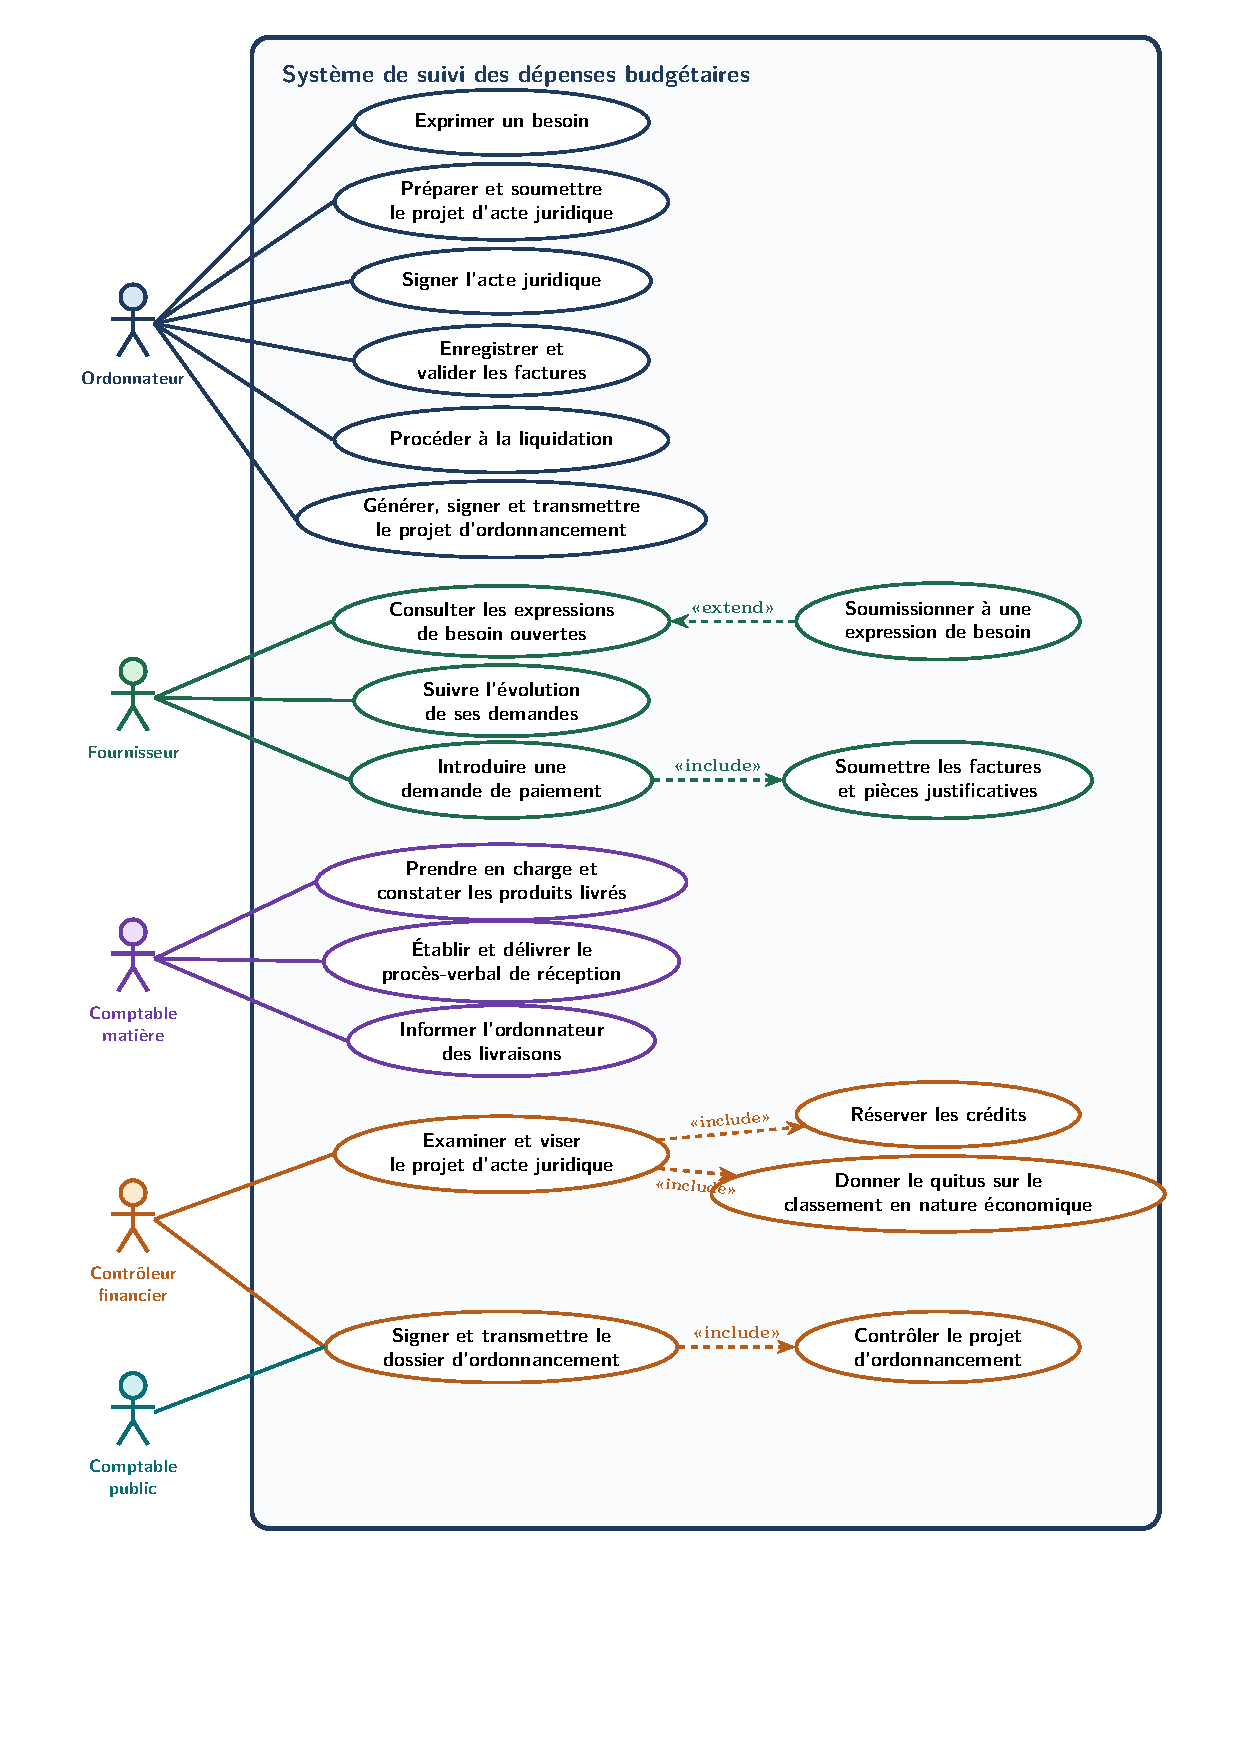
\includegraphics[width=0.98\linewidth,height=0.82\textheight,keepaspectratio]{../diagrammes/cas-utilisation-general.pdf}
\caption{Diagramme général des cas d'utilisation UML — Système de suivi des dépenses budgétaires (fichier source : \texttt{diagrammes/cas-utilisation-general.drawio})}
\label{fig:uc_general}
\end{figure}
\end{landscape}


% 9. Points à clarifier avec le responsable métier
\section{Points à clarifier avec le responsable métier}

Afin de consolider cette première analyse et de préparer les étapes ultérieures de conception (identification des objets métier, définition des cycles de vie et des règles de gestion), plusieurs questions ont été soumises à l'arbitrage du responsable du projet.

\subsection*{Arbitrages métier déjà actés}

À l'issue des premiers échanges de cadrage, les règles de gestion structurantes suivantes sont formellement intégrées à la modélisation :
\begin{itemize}
  \item \textbf{Valorisation de l'expression de besoin :} l'ordonnateur formalise son besoin sous un angle strictement physique et technique (matière, quantités demandées et spécifications techniques). L'attribut de prix unitaire estimé au niveau des lignes de besoin a été supprimé du modèle afin d'éviter toute ambiguïté ou contrainte indue sur l'ordonnateur, la valorisation unitaire relevant exclusivement des offres des soumissionnaires. Aucun plafond strict fondé sur la mercuriale n'est appliqué à ce stade.
  \item \textbf{Soumissions obligatoirement totales :} chaque fournisseur soumissionnaire doit impérativement renseigner un prix unitaire proposé pour chacune des lignes de l'expression de besoin. Les offres partielles ne sont pas admises.
  \item \textbf{Attribution globale :} l'attribution est prononcée au profit d'un prestataire unique pour la totalité de l'expression de besoin.
  \item \textbf{Détermination de la forme de l'acte juridique :} le montant total retenu fixe le seuil légal minimal (interdiction de sous-évaluer ou de recourir à un acte allégé en dépassement de plafond), mais la décision finale intègre la nature économique de la dépense, la durée de la prestation et la décision propre de l'ordonnateur de recourir à un acte plus formalisé pour sécuriser la commande.
\end{itemize}

Les questions subsidiaires ci-après demeurent ouvertes pour les phases d'affinement détaillées.

\subsection{Conditions de publication des expressions de besoin}

\begin{enumerate}
  \item Toutes les expressions de besoin saisies par l'ordonnateur ont-elles vocation à être publiées auprès des fournisseurs, ou certaines dépenses font-elles l'objet d'une procédure restreinte ou directe ?
  \item Une validation interne préalable (hiérarchique ou budgétaire indicative) est-elle requise avant qu'une expression de besoin ne devienne visible comme « ouverte à la soumission » ?
  \item Quelles informations minimales composent une expression de besoin (objet, quantités, spécifications, date limite de soumission, pièces attendues) et selon quelles règles sa clôture intervient-elle ?
\end{enumerate}

\subsection{Processus de sélection des fournisseurs}

\begin{enumerate}
  \item Comment s'opère la transition entre le dépôt des soumissions par les fournisseurs et la préparation du projet d'acte juridique par l'ordonnateur ?
  \item La phase d'examen des offres, de comparaison des soumissions et de sélection du fournisseur retenu doit-elle être gérée et tracée dans l'application, ou relève-t-elle d'une commission externe dont seul le résultat est enregistré ?
  \item Les fournisseurs non retenus doivent-ils être informés via l'application dans le cadre du suivi de leurs demandes ?
\end{enumerate}

\subsection{Modalités de visa et de signature des actes juridiques}

\begin{enumerate}
  \item Dans quel ordre exact interviennent les trois opérations du contrôleur financier lors de l'engagement : la réservation des crédits, le quitus sur le classement des matières dans les natures économiques et le visa du projet d'acte juridique constituent-ils une validation unique ou trois étapes successives distinctes ?
  \item Qui propose initialement le classement des matières dans les natures économiques (l'ordonnateur lors de la préparation du projet d'acte juridique, ou un autre intervenant) avant que le contrôleur financier ne donne son quitus ?
  \item Quelle est la nature exacte de la signature des actes juridiques et des projets d'ordonnancement dans le système (validation électronique interne, signature électronique certifiée ou téléversement d'un document signé manuscritement) ?
  \item Une fois l'acte juridique signé par l'ordonnateur, comment est-il transmis ou notifié au fournisseur retenu pour déclencher les livraisons ?
\end{enumerate}

\subsection{Modalités de réception des livraisons}

\begin{enumerate}
  \item Le fournisseur doit-il déclarer ou annoncer sa livraison dans l'application avant sa prise en charge par le comptable matière, ou l'enregistrement dans le système est-il initié exclusivement par le comptable matière lors de la remise physique des biens ?
  \item De quelle manière le procès-verbal de réception est-il délivré au fournisseur (mise à disposition dans son espace applicatif, notification électronique, remise d'un document signé) ?
  \item L'information de l'ordonnateur par le comptable matière est-elle déclenchée automatiquement dès l'établissement du procès-verbal de réception, ou fait-elle l'objet d'une transmission distincte ?
\end{enumerate}

\subsection{Gestion des livraisons partielles ou non conformes}

\begin{enumerate}
  \item Un même acte juridique peut-il donner lieu à plusieurs livraisons échelonnées (livraisons partielles) donnant chacune lieu à un procès-verbal de réception distinct ?
  \item En cas de livraison partielle, le fournisseur est-il autorisé à introduire une demande de paiement partielle, ou la facturation n'est-elle possible qu'après livraison complète ?
  \item Quelle est la procédure attendue lorsque le comptable matière constate une non-conformité quantitative ou qualitative (procès-verbal de refus ou de réserve, notification au fournisseur et à l'ordonnateur, remplacement des produits) ?
\end{enumerate}

\subsection{Pièces justificatives exigées pour les demandes de paiement}

\begin{enumerate}
  \item Quelle est la liste réglementaire des pièces justificatives que le fournisseur doit soumettre à l'appui de sa demande de paiement et de sa facture ?
  \item Le fournisseur doit-il téléverser à nouveau le procès-verbal de réception et l'acte juridique signé, ou le système les associe-t-il automatiquement au dossier dès lors qu'ils ont été produits dans l'application ?
  \item L'application doit-elle bloquer l'envoi d'une demande de paiement tant que certaines pièces justificatives obligatoires ne sont pas jointes ou tant qu'aucun procès-verbal de réception n'a été enregistré ?
\end{enumerate}

\subsection{Modalités de rejet et de reprise des dossiers}

\begin{enumerate}
  \item Quels sont les différents motifs et niveaux de décision possibles pour le contrôleur financier (tant sur le projet d'acte juridique que sur le projet d'ordonnancement) : visa favorable, rejet définitif ou demande de modification avec renvoi à l'ordonnateur ?
  \item En cas de rejet d'un projet d'acte juridique ou d'un projet d'ordonnancement après réservation des crédits, quel est l'impact sur les crédits réservés (maintien du blocage pendant la correction ou libération automatique des crédits) ?
  \item Lorsque l'ordonnateur invalide une facture soumise par le fournisseur, le dossier retourne-t-il au fournisseur pour régularisation ou donne-t-il lieu à l'introduction d'une nouvelle demande ?
\end{enumerate}

\subsection{Rôle exact du comptable public dans le périmètre de l'application}

\begin{enumerate}
  \item La responsabilité du comptable public dans l'application se limite-t-elle strictement à la réception et à la consultation du dossier d'ordonnancement transmis par le contrôleur financier ?
  \item Le comptable public doit-il pouvoir accuser réception du dossier, enregistrer sa prise en charge comptable, rejeter un dossier incomplet ou renseigner le statut de paiement effectif dans le système ?
  \item Jusqu'à quel jalon exact s'étend la fonctionnalité de suivi des demandes offerte au fournisseur (s'arrête-t-elle à la transmission au comptable public ou inclut-elle l'information du paiement effectif) ?
\end{enumerate}


% 10. Conclusion
\section{Conclusion}

\subsection{Synthèse des acquis de la première étape}

Cette analyse fonctionnelle préliminaire a permis de structurer les besoins exprimés lors de la réunion de cadrage initial autour d'une vision cohérente du système de suivi des dépenses budgétaires :

\begin{itemize}
  \item le processus métier a été organisé en quatre phases lisibles couvrant l'ensemble de la chaîne, de l'expression du besoin à la transmission du dossier d'ordonnancement au comptable public ;
  \item les cinq acteurs du système (\emph{Ordonnateur}, \emph{Fournisseur}, \emph{Contrôleur financier}, \emph{Comptable matière} et \emph{Comptable public}) ont été caractérisés avec précision, en distinguant leurs responsabilités métier réglementaires des futurs droits d'accès applicatifs ;
  \item le périmètre fonctionnel a été traduit en dix-neuf cas d'utilisation répartis en quatre domaines et représentés dans un diagramme général UML respectant strictement la notation standard.
\end{itemize}

\subsection{Prochaines étapes de conception}

Ce document de travail a désormais vocation à être examiné et validé par le responsable du projet. Les réponses apportées au questionnaire de clarification (section 8) permettront d'engager la seconde étape des travaux d'analyse et de conception, qui portera sur :

\begin{enumerate}
  \item la description textuelle détaillée des scénarios nominaux et alternatifs de chaque cas d'utilisation (notamment la gestion des rejets, des régularisations et des livraisons partielles) ;
  \item l'identification des principaux objets métier du domaine, de leurs attributs et de leurs cycles d'états (diagramme de classes du domaine métier) ;
  \item la définition de la matrice fine des habilitations par profil d'utilisateur.
\end{enumerate}


\end{document}
